\documentclass[a4paper,12pt,twoside]{../includes/ThesisStyle}
\usepackage[utf8]{inputenc}
\usepackage[T1]{fontenc}

\usepackage[left=1.5in,right=1.3in,top=1.1in,bottom=1.1in,includefoot,includehead,headheight=13.6pt]{geometry}\renewcommand{\baselinestretch}{1.05}


% =============================================================================
%\usepackage[sectionbib]{chapterbib}	% Cross-reference package (Natural BiB)
%\usepackage{bibunits}
%\usepackage{natbib}					% Put References at the end of each chapter
\usepackage{algorithm}
\usepackage{alltt}
\usepackage{amsfonts}
\usepackage{amsmath}
\usepackage{amssymb}
\usepackage{cite}
\usepackage{color}
\usepackage{enumerate}
\usepackage{booktabs} % used for \midrule
\usepackage{fancyhdr}					% Fancy Header and Footer
\usepackage{graphicx}
\usepackage{ifthen}
\usepackage{latexsym}
\usepackage{multirow}
\usepackage{rotating}					% Sideways of figures & tables
\usepackage{stmaryrd}
\usepackage{subfigure}
\usepackage{url}         
\usepackage{xspace}
\usepackage[normalem]{ulem} % for \sout
\usepackage{xcolor}
\usepackage{tablefootnote}
\usepackage{pifont}

% =============================================================================

% Table of contents for each chapter
\usepackage[nottoc, notlof, notlot]{tocbibind}
\usepackage{minitoc}
\setcounter{minitocdepth}{1}
\mtcindent=15pt

\setcounter{secnumdepth}{3}
\setcounter{tocdepth}{2}
  
% =============================================================================
% Fancy Header Style Options

\pagestyle{fancy}                       % Sets fancy header and footer
\fancyfoot{}                            % Delete current footer settings

%\renewcommand{\chaptermark}[1]{         % Lower Case Chapter marker style
%  \markboth{\chaptername\ \thechapter.\ #1}}{}} %

%\renewcommand{\sectionmark}[1]{         % Lower case Section marker style
%  \markright{\thesection.\ #1}}         %

\fancyhead[LE,RO]{\bfseries\thepage}    % Page number (boldface) in left on even
% pages and right on odd pages
\fancyhead[RE]{\bfseries\nouppercase{\leftmark}}      % Chapter in the right on even pages
\fancyhead[LO]{\bfseries\nouppercase{\rightmark}}     % Section in the left on odd pages

\let\headruleORIG\headrule
\renewcommand{\headrule}{\color{black} \headruleORIG}
\renewcommand{\headrulewidth}{1.0pt}
\usepackage{colortbl}
\arrayrulecolor{black}

\fancypagestyle{plain}{
  \fancyhead{}
  \fancyfoot{}
  \renewcommand{\headrulewidth}{0pt}
}


% =============================================================================
% Clear Header Style on the Last Empty Odd pages
\makeatletter

\def\cleardoublepage{\clearpage\if@twoside \ifodd\c@page\else%
  \hbox{}%
  \thispagestyle{empty}%              % Empty header styles
  \newpage%
  \if@twocolumn\hbox{}\newpage\fi\fi\fi}

\makeatother

\newenvironment{maxime}[1]
{
\vspace*{0cm}
\hfill
\begin{minipage}{0.5\textwidth}%
%\rule[0.5ex]{\textwidth}{0.1mm}\\%
\hrulefill $\:$ {\bf #1}\\
%\vspace*{-0.25cm}
\it 
}%
{%

\hrulefill
\vspace*{0.5cm}%
\end{minipage}
}

\let\minitocORIG\minitoc
\renewcommand{\minitoc}{\minitocORIG \vspace{1.5em}}


\renewcommand{\epsilon}{\varepsilon}

% centered page environment
\newenvironment{vcenterpage}
	{\newpage\vspace*{\fill}\thispagestyle{empty}\renewcommand{\headrulewidth}{0pt}}
	{\vspace*{\fill}}
	

%=============================================================================

\usepackage{needspace}
\newcommand{\needlines}[1]{\Needspace{#1\baselineskip}}

\usepackage{xcolor}
\definecolor{source}{gray}{0.95}
% source code formatting
\usepackage{listings}
    % global settings for source code listing package
\lstset{
    basicstyle=\ttfamily\small,
    showspaces=false,
    showstringspaces=false,
    captionpos=b, 
    columns=fullflexible}

\lstdefinelanguage{ST}{
    keywordsprefix=\#,
    morekeywords=[0]{true,false,nil},
    morekeywords=[1]{self,super,thisContext},
    morekeywords=[2]{ifTrue:,ifFalse:,whileTrue:,whileFalse:,and:,or:,xor:,not:,by:,timesRepeat:},
    sensitive=true,
    morecomment=[s]{"}{"},
    morestring=[d]',
    escapechar={!},
    alsoletter={., :, -, =, +, <},
    moredelim=**[is][\itshape]{/+}{+/},
    literate=
        {^}{{$\uparrow$}}1
        {:=}{{$\leftarrow$}}1
        {~}{{$\sim$}}1
        {-}{{\sf -\hspace{-0.13em}-}}1  % the goal is to make - the same width as +
        {+}{\raisebox{0.08ex}{+}}1		% and to raise + off the baseline to match V
        , % Don't forget the comma at the end!
    style=STStyle
}
\lstdefinestyle{STStyle}{
    tabsize=4,
    %frame=leftline,
    % frame=bl,
    %framerule=2pt,
    %rulecolor=\color{gray},
    % backgroundcolor=\color{white},
    %backgroundcolor=\usebeamercolor[bg]{listing},
    basicstyle=\ttfamily\small,
    keywordstyle=\bf\ttfamily,
    % stringstyle=\color{orange},
    stringstyle=\mdseries\slshape,
    commentstyle=\it\rmfamily\color{darkgray}, 
    commentstyle=\mdseries\slshape\color{gray},
    %commentstyle=\mdseries\slshape,
    emphstyle=\bf\ttfamily,
    escapeinside={!}{!},
	%backgroundcolor=\color{source},
    %emphstyle={[2]\color{red}},
    %emphstyle={[3]\color{blue}\bf},
    %emphstyle={[4]\color{blue}},
    keepspaces=true
} 

%\lstnewenvironment{javacode}  [1][]{\lstset{language=java,#1}\needlines{#2}}{} 
%\lstnewenvironment{pythoncode}[2][]{\lstset{language=python,#1}\needlines{#2}}{}
\lstnewenvironment{stcode}    [2][]{\lstset{language=ST,#1}\needlines{#2}}{}
\lstnewenvironment{ccode}     [2][]
    {\lstset{language=C,numbers=left,escapechar=\$,numberstyle=\tiny,#1}\needlines{#2}}{}

% ON: I tried to pass the line number options in as arg #1 but it does not work for me
% I also could net get the line numbers to consistently increase
\lstnewenvironment{numstcode} [2][]
    {\lstset{language=ST,numbers=left,numberstyle=\tiny,numbersep=2pt,#1}\needlines{#2}}{}
\lstnewenvironment{numstcodecont} [2][]
    {\lstset{language=ST,numbers=left,numberstyle=\tiny,numbersep=2pt,firstnumber=last#1}\needlines{#2}}{}

\newcommand{\lst}[1]{{\tt #1}}

% In-line code (literal)

% In-line code (latex enabled)
% Use this only in special situations where \ct does not work
% (within Section headings ...):
\newcommand{\lct}[1]{{\textsf{\textup{#1}}}}
% Code environments
\lstnewenvironment{code}{%
	\lstset{%
		% frame=lines,
		frame=single,
		framerule=0pt,
		mathescape=false
	}
}{}

%\renewcommand{\lstlistingname}{Code Example}

% =============================================================================
\newboolean{showcomments}
\setboolean{showcomments}{true}

\ifthenelse{\boolean{showcomments}} {
	\newcommand{\ugh}[1] {\textcolor{red}{\uwave{#1}}}	% please rephrase
	\newcommand{\ins}[1] {\textcolor{blue}{\uline{#1}}}	% please insert
	\newcommand{\del}[1] {\textcolor{red}{\sout{#1}}}	% please delete
	\newcommand{\chg}[2] {								% please change
		\textcolor{red}{\sout{#1}}{\ra}
		\textcolor{blue}{\uline{#2}}}
	\newcommand{\nbc}[3]{								% comment
		{\colorbox{#3}{\bfseries\sffamily\scriptsize\textcolor{white}{#1}}}
		{\textcolor{#3}{\sf\small$\blacktriangleright$\textit{#2}$\blacktriangleleft$}}}

}{
	\newcommand{\ugh}[1]{#1}							% please rephrase
	\newcommand{\ins}[1]{#1}							% please insert
	\newcommand{\del}[1]{}								% please delete
	\newcommand{\chg}[2]{#2}							% please change
	\newcommand{\nbc}[3]{}								% comment
}

% =============================================================================
\usepackage[pagebackref,hyperindex=true]{hyperref}


% Links in pdf
\usepackage{color}
\definecolor{linkcol}{rgb}{0.0, 0.0, 0.0} 
\definecolor{citecol}{rgb}{0.0, 0.0, 0.0} 

% Change this to change the informations included in the pdf file
% See hyperref documentation for information on those parameters
\hypersetup {
	bookmarksopen=true,
	pdftitle="Design and Use of Anatomical Atlases for Radiotherapy",
	pdfauthor="Olivier COMMOWICK", 
	pdfsubject="Creation of atlases and atlas based segmentation", %subject of the document
	%pdftoolbar=false, % toolbar hidden
	pdfmenubar=true, %menubar shown
	pdfhighlight=/O, %effect of clicking on a link
	colorlinks=true,
	pdfpagemode=UseNone,
	pdfpagelayout=SinglePage,
	pdffitwindow=true,
	linkcolor=linkcol,
	citecolor=citecol,
	urlcolor=linkcol
}

% =============================================================================
\newcommand{\figlabel}[1] {\label{fig:#1}}
\newcommand{\chaplabel}[1]{\label{chap:#1}}
\newcommand{\seclabel}[1] {\label{sec:#1}}
\newcommand{\tablabel}[1] {\label{tab:#1}}
\newcommand{\lstlabel}[1] {\label{lst:#1}}

\newcommand{\figref}[1] {Figure~\ref{fig:#1}}
\newcommand{\chapref}[1]{Chapter~\ref{sec:#1}}
\newcommand{\secref}[1] {Section~\ref{sec:#1}}
\newcommand{\tabref}[1] {Table~\ref{tab:#1}}
\newcommand{\lstref}[1] {Listing~\ref{tab:#1}}

\newcommand{\commented}[1]{}

\newcommand{\bs}    {\symbol{'134}} % backslash
\newcommand{\us}    {\symbol{'137}} % underscore
\newcommand{\ttt}[1]{\texttt{#1}}
\newcommand{\ie}    {\emph{i.e.},\xspace}
\newcommand{\eg}    {\emph{e.g.},\xspace}
\newcommand{\etal}  {\emph{et al.}\xspace}
\newcommand{\ns}    {\!\!\!\!} %big negative space
\newcommand{\cnull} {\textbackslash0\xspace}


\newcommand\fix[1]{\nb{FIX}{#1}}
\newcommand\todo[1]{\nb{TO DO}{#1}}
\newcommand\cb[1]{\nbc{CB}{#1}{purple}}
\newcommand\sd[1]{\nbc{SD}{#1}{orange}}
\newcommand\is[1]{\nbc{IS}{#1}{gray}}
\newcommand\gc[1]{\nbc{GC}{#1}{olive}}
\newcommand\ct[1]{\nbc{CT}{#1}{teal}}
\newcommand\md[1]{\nbc{MD}{#1}{blue}}
\newcommand\dc[1]{\nbc{DC}{#1}{green}}

% =============================================================================
\newcommand{\NBFFI}  {Native\-Boost-FFI\xspace}
\newcommand{\NB}  {Native\-Boost\xspace}
\newcommand{\B}   {Benzo\xspace}
\newcommand{\ST}  {Small\-talk\xspace}
\newcommand{\PH}  {Pharo\xspace}
\graphicspath{{.}{../figures/}}

\begin{document}
% ===========================================================================

\chapter{\B Prototype Application Validation}
\chaplabel{validation}
\minitoc
% ===========================================================================
\introduction
% ===========================================================================

In \chapref{ffi} we presented \NB, a mature language-side \FFI implementation that makes heavy use of \B's infrastructure.
\NB is only one of three applications that are based on \B that were initially outlined in \secref{benzo-usecase}.
While \NB is considered stable, the two other applications are currently only prototypes: dynamic primitives and a language-side \JIT.
Hence we will present the two solutions combined in this chapter.

As first we will present \WF, dynamic primitives based on \B.
\WF takes advantage of the metacircular approach of \PH's \VM and makes the primitive definition available at runtime.
This is a step forward from the typical metacircular approach where the whole reflective power of the host environment can only be used at compile-time.
Once the \VM is compiled, all the high-level definitions that existed at compilation time are no longer accessible from language-side.
\WF tries to make a fraction of the original compile-time definitions accessible.

\todo{probably retrofit to the final results of \NBJ}\enlargethispage{\baselineskip}
The second prototype, \NB a language-side \JIT compiler takes the core idea of \WF even further.
\WF is capable of defining new primitives at runtime which are not reentrant: it is not possible to activate \PH methods from within primitives.
However, this is what happens in jitted methods: it is possible to switch seamlessly between native methods and standard \PH methods using bytecode evaluation.
Much like the primitives, the \JIT can not be changed from language-side and this is where we bring \NBJ into play.
\NBJ reimplements the \VM-level \JIT compiler at language-side and uses \B to install the native code.


% ===========================================================================
%\newpage
\section{\WF: Dynamic Primitives}
\seclabel{val-waterfall}
% ===========================================================================

\begin{figure}[h]
	\centering
	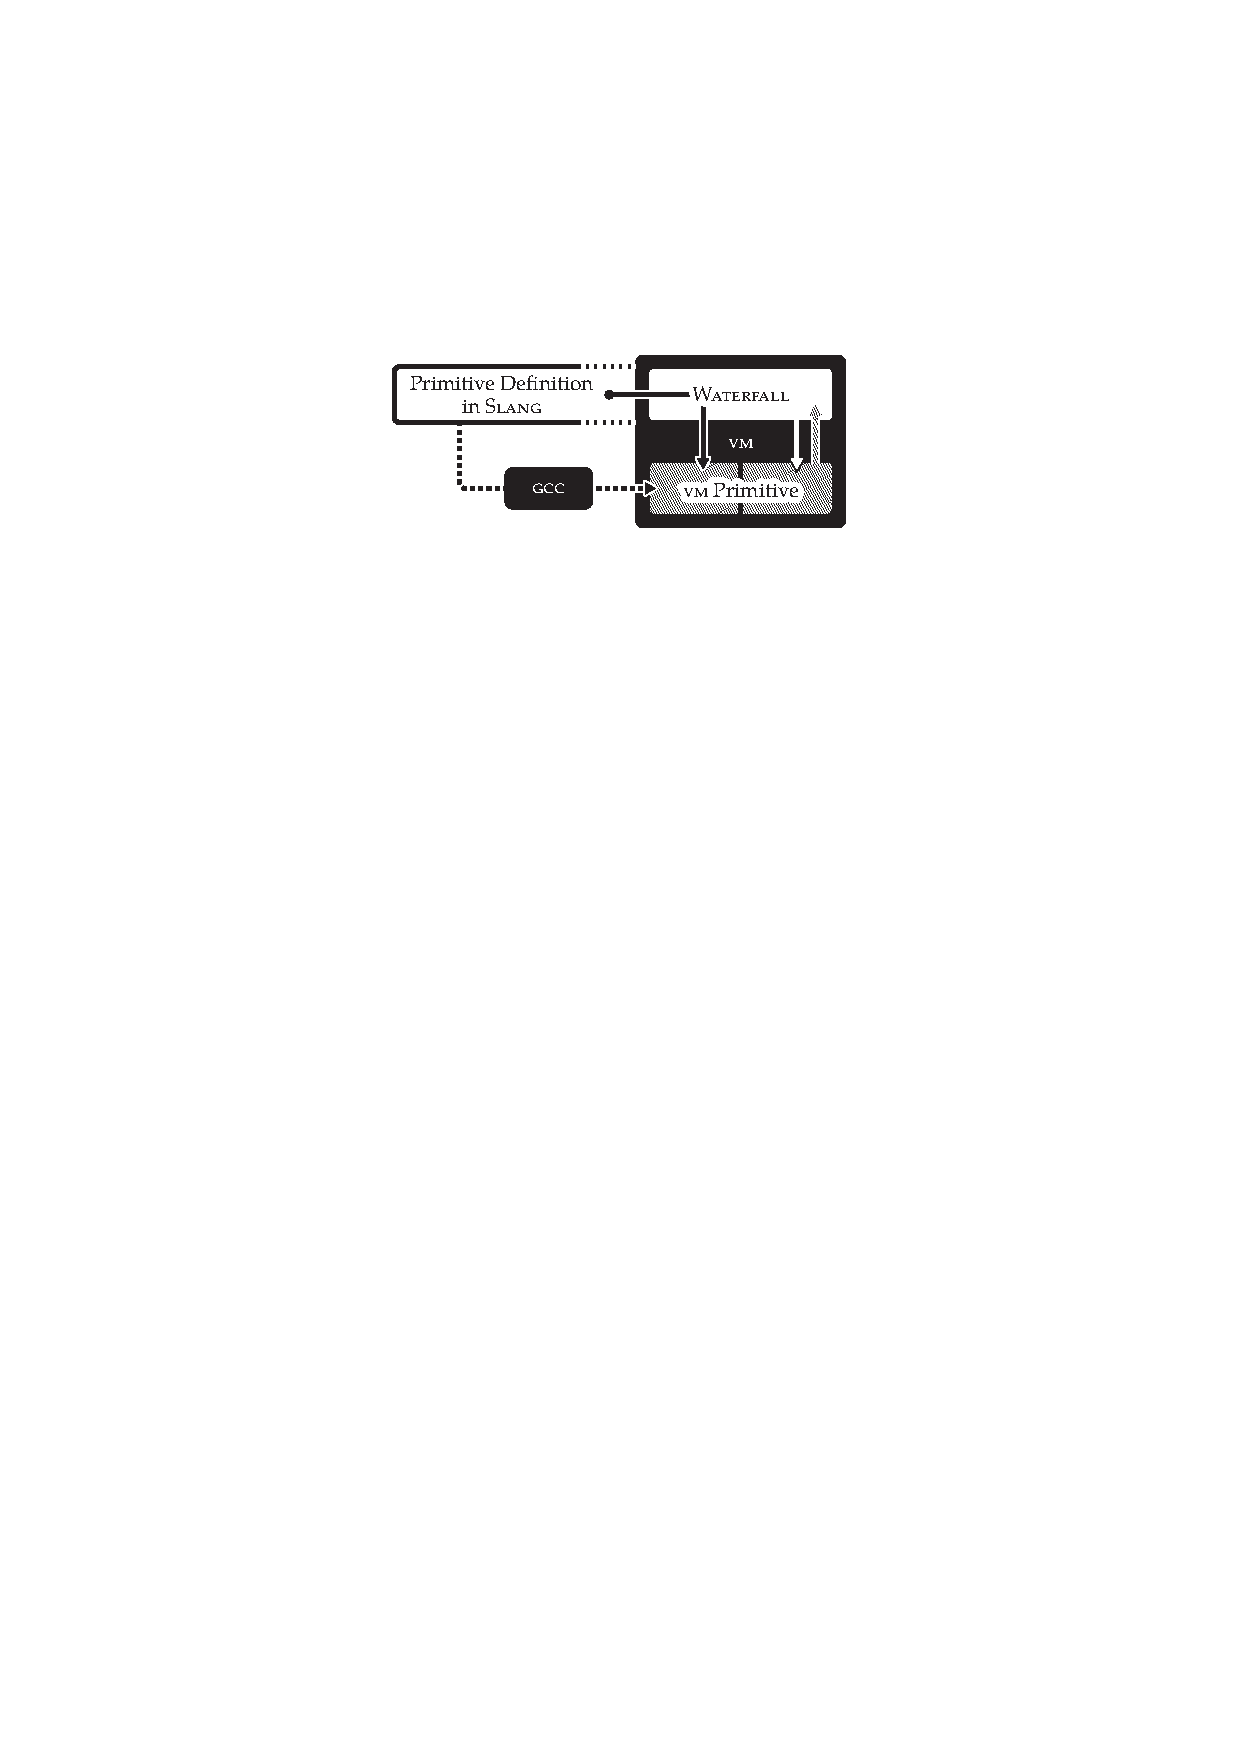
\includegraphics[scale=\imagescale]{waterfall-overview}
	\caption{\WF Overview}
	\figlabel{val-waterfall-overview}
\end{figure}

\noindent In this section we present \WF, a compiler toolchain that allows primitives to be changed dynamically from language-side.
We successfully use \WF to change and recompile whole \VM plugins such as the file plugin as we show in the following \secref{val-waterfall-plugins}.

% -----------------------------------------------------------------------------
\subsection{Background}
\seclabel{val-waterfall-background}
% -----------------------------------------------------------------------------

\WF is our second application on top of \B after \NB, the complete \FFI library previously presented in \chapref{ffi}.
\NB uses \B to generate the glue code between \PH and the external library.
Even though \NB is extendable it is not used to directly synthesize new functionality, the main functionality is defined the external libraries typically written in a low-level language such as C.
Interestingly, the \NB methods containing the callouts behave almost like the existing primitive methods of \PH.
These primitives define a hook into \VM-level native functionality.
In \PH the same mechanism is also used to activate plugins which are again similar to an \FFI callout from language-side.
However, primitives and plugins are statically defined and modifications happen outside \PH.
This is where the domain of \WF begins.

\WF provides infrastructure to dynamically compile and install primitives on top of the \B infrastructure at language-side in \PH.
As we will describe in more detail in the following sections, the \PH \VM is written in a metacircular fashion.
Hence the definition of plugins and primitives can be loaded in standard \PH.
Typically this happens only at compile-time of the \VM, where these definitions are exported to C and compiled to the \VM binary.
Once compiled, the original high-level description of primitives and plugins is no longer accessible from \PH.
As a consequence, existing primitives or plugins can not be changed at runtime.

\WF brings the static primitive definitions to live again.
Just loading the original definitions in \PH does not bring them back to live, even though we can now inspect the definition and browse the sources.
\WF compiles these definitions to native code and installs them with \B as new primitives.
With this infrastructure primitive and plugin modifications are not limited to \VM compilation time.

\paragraph{A Metacircular \VM Written in \Slang}

\WF is implemented in \PH which uses the \urlfootnote{\Cog \VM}{http://www.mirandabanda.org/cogblog/}, originating from the \Squeak \VM\cite{Inga97a}.
The \VM itself is written in a dialect of \ST called \Slang that is essentially limited to the functionality that can be expressed with standard C code.
\Slang serves for two purposes: a high-level C preprocessor, a interactive simulator of the \VM.
The first point has severe consequences.
\Slang basically has the same syntax as \ST but is semantically constrained to expressions that can be resolved statically at compilation or code generation time and are compatible with C.
Hence \Slang's semantics are closer to C than to \ST.
This fact is also visible in the simulator for the \VM.
If \Slang were \ST, separate parts of the \VM could be directly evaluated.
However, since \Slang is bound to C expressions, the simulator sets up a byte array as memory.
The simulated \VM then accesses this byte array as if it were the native memory.

In conclusion we see that the \PH \VM has an abstract representation of the \VM available for simulation.
This abstract representation is then used to generate C sources, already lowering the abstraction level.
After compiling the C sources the original representation of the \VM is not directly accessible anymore.
For instance, even debug symbols are usually stripped from the final binary for performance reasons.
Of course this implies that the \VM can not be changed nor directly inspected from language-side.


\paragraph{Primitives in \PH}
\PH is a highly reflective environment where classes and methods can be changed at runtime, even the current execution context is accessible.
For instance this is used to implement an exception mechanism purely at language-side in \PH.
However, some features can not be implemented at language-side.
\PH uses primitive methods, that instead of evaluating \PH-code switch to a \VM routine.
As already partially explained in \secref{benzo-vm-interaction}, whenever a method is compiled with the \ttt{primitive} pragma as shown a flag is set on the \ttt{CompiledMethod}. 
If the \VM tries to activate such a method, instead of interpreting the bytecodes it calls the corresponding function at \VM-level~\cite{Gold83a}.
We distinguish three categories of primitives based on their functionality: certain parts of the language semantics, \OS-level functionality that can not be implemented in \PH itself and a third less important category where performance is critical.

As we mentioned in the previous paragraph, these primitives are bound to the \VM and can not be changed at runtime.
However, for a certain subset of these primitives we can write language-side substitutes in pure \PH-code.
These primitives are called non-essential and are mainly used for optimization purposes. 
In contrast there are essential primitives which are for instance used during start up of the \PH environment.
Two prominent examples of essential primitives are the ones used for creating new objects or activating a block.

\paragraph{Instrumenting Primitives}
In the context of \WF we are interested in which parts of the system we can modify and thus we draw our attention to these essential primitives.
The only way to modify these primitives is by creating wrappers but that brings a new problem.
Imagine that we wrap around the primitive which creates a new object.
What happens now if the additional wrapper code needs a new object?
It will call the very same primitive that we just wrapped, without protection this causes infinite recursion.
Since technically the wrapper code should live at a different abstraction level than the original primitive we have find our selves mixing meta-levels \cite{Chib96a}.

The most radical approach to avoid this meta-recursion is to change the primitive externally.
In the case of \PH this means changing the \Slang sources, exporting and compiling the primitive and restarting the \PH environment on top of this changed \VM.
However, this approach stands in contrast to the reflective nature of \PH where most functionality can be changed at runtime.
Also it is not always suitable to restart the \PH process to modify a small part of the system.

%----------------------------------------------------------------------------
\subsection{\WF's Contribution}
Following the implementation overview of the \PH \VM and the differentiation of different primitives we identify two main benefits of changing \VM primitives at runtime with \WF:

\begin{enumerate}
	\item Reducing \VM complexity by implementing non-essential primitives reflectively at language-side.
	\item Dynamic instrumentation of primitives.
\end{enumerate}

\paragraph{Reducing \VM Complexity}
Low-level \VM extensions are only justified in the presence of strong performance requirements (see \secref{benzo-related}).
All non-essential primitives fall into this category since these primitives can be implemented in \PH without restrictions.
However, in certain cases for performance a language-side implementation is unsuitable.
Additionally we already know that these primitives are available as \Slang code at \VM generation time.
Using \WF, these primitives can be implemented at language-side based on the unmodified \Slang sources.
This means that these primitives become first-class citizens of the high-level environment and thus evolve with less effort.
Thus, \WF opens new possibilities of changing \PH that were previously possible only with significant overhead.

\paragraph{Essential Primitives}
For essential primitives the previous argument does not hold since a static version is needed for a correct startup of the system.
These primitives can not be directly replaced by a language-side implementation using \WF.
Even though \WF itself avoids meta-recursion by generating low-level code with \B.
However, \B itself relies on essential primitives as it is written in \PH.
This imposes certain restrictions how and when these essential primitives can be modified with \WF during system startup.
These restrictions are more related to the underlying \B infrastructure than \WF.
For instance already exposed similar limitations with the \B-based \FFI when used during startup (see \secref{ffi-startup-recursion}).
Nevertheless, nothing prevents from replacing essential primitives at runtime with customized versions, once the system startup is completed. 

\paragraph{Extended Primitive Instrumentation}
Instrumentation of essential primitives from lan\-guage-side is an error-prone task falling in many cases in non-termination due to previously described meta-recursion. 
An example of this behavior, can be observed when changing the essential \ttt{basicNew} primitive, which is responsible for instantiating new objects.
Only very limited instrumentation is possible at language-side, for instance counting how many instances have been created.
This only works since the \VM internally does not represent small integers as full objects.
However, this is only true up to some extent.
Small integers bigger than $2^{30}$ are transformed to a more expensive object representation since they no longer fit in a machine word of the 32-bit \VM. 
These big integers will use the \ttt{basicNew} primitive again as they are not implement in the \VM but in at language-side.
Thus, we are back the original problem of running into meta-recursion.
So even this very simple example has unwanted side-effects that are not directly visible.
More complex instructions tasks will inevitably suffer from the same problems.

Using reflective techniques it is possible to escape from this meta-recursion, however, with a considerable overhead.
\WF avoids these issues since the instrumentation code for primitives will be implemented at the lowest level on top of \B.
In \secref{val-waterfall-performance} we show how \WF, the \B based approach for generating primitives on the fly, outperforms the reflective solutions for primitives instrumentation. 


% -----------------------------------------------------------------------------
\subsection{\WF Implementation}
\seclabel{val-waterfall-implementation}
% -----------------------------------------------------------------------------
\WF uses \B's mechanism for replacing primitive methods with customized versions that are nativized dynamically as described in \chapref{benzo}.
The loophole described there is exploited by \WF to enable dynamic modification of \VM behavior and hence bring primitives to life at language-side.
From a high-level point of view \WF provides two services which work transparently: 

\begin{enumerate}
	\item Compilation of \Slang code on demand (lazily).
	\item A clear interface for executing, at runtime and from language-side, the native code generated.
\end{enumerate}

\noindent The first item allows to change the code of primitives at language-side and generate the corresponding native code when needed. 
It also provides the possibility to write methods or functionality with the same \ST syntax but with a static semantic. 
It consists essentially of a transformation toolchain that transforms the \Slang sources to native code using a \B-based compilation toolchain.

The second item enables the execution of the dynamically generated native code.
This includes for instance the finding of addresses of \VM internal symbols and all the effort to link the two worlds, \ST and native.
\WF relies on \B for most of this low-level functionality.
In particular \NB, the \B-based \FFI presented in \chapref{ffi}, is used for interfacing with C libraries (\ttt{dlsym}). 

% -----------------------------------------------------------------------------
\paragraph{Architecture Overview}
The \WF infrastructure is mainly divided in the following two parts: 
\begin{itemize}[nolistsep,noitemsep]
	\item the installed \Slang sources,
	\item a \B-based compilation toolchain.
\end{itemize}
The \WF compiler transforms the \Slang sources to native code through various transformation steps as show in \figref{waterfall-architecture}.
In order to work properly \WF needs the complete \Slang sources for compilation unit (primitive or plugin) to be loaded upfront.
Once loaded in the \PH image the \AST of the \Slang sources are available which form the input for the \WF compiler.
This means that it is possible to write custom plugins in \PH and transform them using \WF as long as the written \PH code uses the restricted \Slang subset.
As mentioned earlier, the major difference to normal \PH code is the lack of real polymorphism since \Slang is more like C with a \ST syntax.

Technically the \WF compiler takes over the part of the \Slang to C converter and of \GCC in the normal \VM compilation process.
\WF, much like the \Slang to C converter, has to take care of certain type information present in the \Slang sources.
For instance we extract from the type information if arguments are used by value or reference.
With this information we generate native code using a simple stack based strategy for temporary variables.
As for the part of \GCC, \WF in its current state is of course far less complex and the resulting the native code is inferior to \GCC's optimized output.
To simplify the prototype \WF only uses a simple stack strategy instead of register allocation for temporaries.
Additionally \WF does not use intermediate representations (\IR) such as static single assignment (\SSA) to perform elaborate optimizations \cite[Ch.\ 1]{Appe98a}.


% -----------------------------------------------------------------------------
\paragraph{Compilation Steps}
As shown in \figref{waterfall-architecture} the \WF compiler transforms the \AST of the \Slang input to \PH primitives.

\begin{figure}[h]
	\centering
	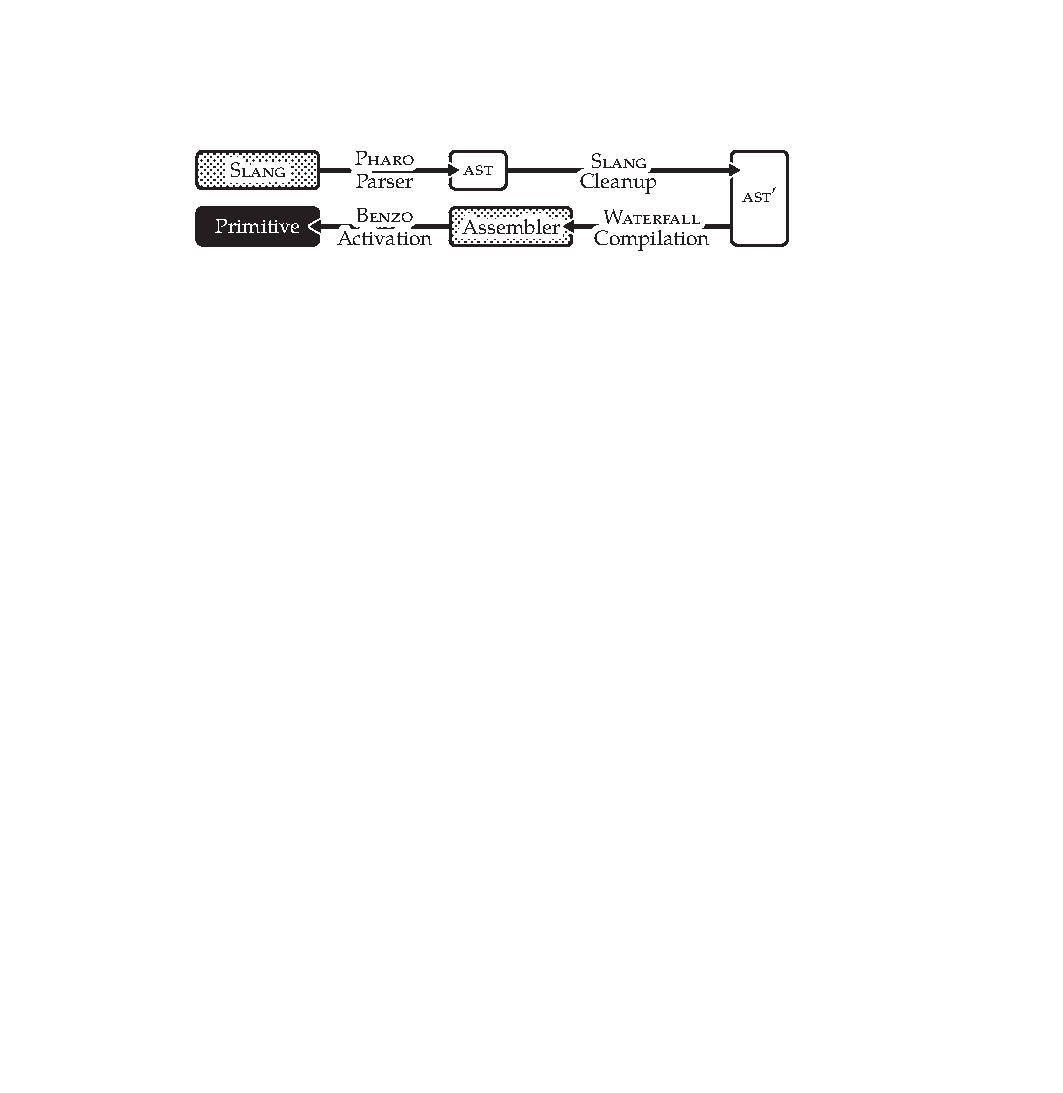
\includegraphics[scale=\imagescale]{waterfall-architecture}
	\caption{\WF Compilation Steps}
	\figlabel{waterfall-architecture}
\end{figure}

\noindent We divide the \WF compiler into four distinct steps:
\begin{description}
\item[\Slang to \AST:] The first step is to access the \AST of the \Slang source method which happens automatically by loading the \Slang code in the \PH image.
At this stage \WF also recursively collects the set of reachable \Slang methods.


\item[\AST Purification:] In a second step certain expressions of the original \Slang \AST are transformed into custom \WF expressions that can be easier transformed later on.
For instance \WF converts C macros that are supported in \Slang which of course only make sense when using a standard C compiler.

\item[\AST to \ASM:] The real native compilation happens in the third step where an \AST-visitor creates assembler instructions using \B's \AsmJIT.
At this point external symbols are statically resolved and directly inlined in the final \ASM code.

\item[\ASM to Primitive] Although not strictly part of the compilation, in the fourth step the final native instructions are installed as a primitive methods using \B (see \secref{benzo-benzo} for more details).
\end{description}


% -----------------------------------------------------------------------------
\paragraph{Dynamically Replacing Primitives}
After explaining the general architecture and the different compilation steps of \WF we shed some light on how the primitives are actually installed.
In reality we rely 100\% on \B for this feature.
Once the native code is generated we transform the target method to a special \B-enabled method that contains the native code.
This procedure is explained in detail in \secref{benzo-benzo} where we show the implementation details of \B.

From a user point-of-view we only have to make sure that the corresponding \Slang sources are available and then hand over that source method to \WF to compile and install it.
Once the installation is complete, the resulting \B-enabled method will contain behave like a \Slang primitive compiled with the original approach using \GCC.

% -----------------------------------------------------------------------------
\paragraph{Dynamically Replacing Plugins}
In \PH there is no real distinction between primitives and plugins as we illustrate with the following code snippets.
The first one depicts an essential primitive to allocate new objects.
The second code example shows the a plugin primitive to open a new file stream.
%
\begin{stcode}[
	caption={\ttt{Object>>\#basicNew} Primitive},
	label={lst:validation-basicnew}]{3}
basicNew
  <primitive: 70>
  OutOfMemory signal.
\end{stcode}
%
\begin{stcode}[caption={\ttt{FilePlugin>>\#open:writeable:} Plugin Primitive}]{5}
open: pathString writable: writableFlag
  "Open a file at the given pathString, and return
   the file ID obtained."
  <primitive: 'primitiveFileOpen' module: 'FilePlugin'>
  ^ nil
\end{stcode}
%
The main difference between primitives and plugins is only how they are distributed.
Primitives are inlined in the \VM and can not be loaded at runtime, while plugins can be loaded dynamically and are bundled separately.
That also means that there is no difference in handling plugins for \WF, the compilation and installation process is exactly the same.

% -----------------------------------------------------------------------------
\subsection{\WF Validation}
\seclabel{val-waterfall-performance}
% -----------------------------------------------------------------------------
After explaining the implementation details of \WF we would like to present a thorough evaluation of the \WF infrastructure.
We split up the validation in two parts following the outlined applications of \WF in the introduction.
The first part describes the performance of \WF when used for instrumenting primitives.
This is the major field of application for \WF as it stresses its dynamic nature.
In contrast to that we evaluate the performance of a \WF compiled plugin in the second part of the validation.
Evaluating a whole plugin puts more stress on the quality of the generated code than the fact that we can dynamically modify primitives.
A more detailed analysis of \WF is also available separately \cite{Char13a}.


% -----------------------------------------------------------------------------
\subsubsection*{Validation of Dynamic Primitives}

In this first part of the \WF validation we compare the performance of \WF generated primitives in \PH.
In the first part we simply measure the speed of a dynamically replaced primitive, while in the second we add instrumentation overhead.
For the simple replacement we choose the simple integer operation "greater than" (\ttt{$>$}) and for instrumentation the more complex \ttt{basicNew} primitive.

\paragraph{Simple Dynamic Primitives}
In this first validation we compare the speed of the \WF generated code on a simple "greater than" primitive.
The primitive is rather simple as it only works on small integers arguments and delegates the functionality for other types to its superclass.
The code for the \ttt{SmallInteger} operation looks as follows.
%
\begin{stcode}{3}
> aNumber
	<primitive: 4>
	^super > aNumber
\end{stcode}
%
The fallback code at the end of the method triggers a slower "greater than" implementation on the super class \ttt{Integer} which mostly deals with the multitude of possible arguments to \ttt{>}.

\begin{stcode}{1}
> aNumber
	aNumber isInteger 
		ifFalse:[
			^ aNumber 
				adaptToInteger: self andCompare: #> ]
	self negative == aNumber negative
		ifFalse: [ ^ aNumber negative ].
	self negative
		ifTrue: [ ^(self digitCompare: aNumber) < 0 ]
		ifFalse: [ ^(self digitCompare: aNumber) > 0 ].
\end{stcode}


\noindent For comparing performance of the "greater than" primitive we use three different approaches:
%
\begin{enumerate}[noitemsep,nolistsep]
	\item the standard primitive provided by the \VM,
	\item the fallback language-side implementation that is triggered whenever the standard primitive failed,
	\item the reimplementation with \WF (not instrumented).
\end{enumerate}
%
We run the three approaches by measuring the cumulative time over one million primitive activations averaged over $100$ runs.
The absolute numbers are less important than the relative factor between them.
We present the results of this experiment in ~\tabref{val-waterfall-performance}.
%
\begin{table}[H]
    \centering
    \begin{tabular}{rSS}
					& {Running Time [ms]} & {Relative Time} \\\midrule
		Unmodified	&   6.4(14)           & 1.0\\
		Fallback	& 195.0(16)           & \approx30.0 \\
		\WF	        &  22.8(17)           & \approx3.6
    \end{tabular}
    \caption[\WF Speed Comparison: Large Integer]{Comparing running time of different implementations of integer arithmetic primitive.}
    \tablabel{val-waterfall-performance}
\end{table}

\noindent As expected \WF's solution outperforms pure reflective one by factor $9$ to $10$.
\WF clearly outperforms a purely reflective solution since all the meta programming overhead for the intercession mechanism is avoided.
This results thus makes a whole new set of runtime extensions feasible that were previously limited by their strong performance penalty.
Furthermore the performance penalty over a completely optimized \VM solution that has extreme optimization techniques, such as inlining and register allocation, is less than a factor of $4$.

\paragraph{Essential Primitive Instrumentation}
As a second validation target for primitives we chose to instrument \ttt{basicNew} which is a critical primitive for object allocation.
Like the previous "greater than" primitive this belongs to the set of essential primitives that are used during startup of the image.
For instrumentation \ttt{basicNew} is again a rather tricky target as wrong code easily leads to infinite recursion.
However, this can be avoided with a rather costly recursion guard.
We chose a rather simple instrumentation method by simply printing the address of the allocated object to the standard output stream.
We validate the four flavors of the \ttt{basicNew} primitive:
\begin{enumerate}[noitemsep,nolistsep]
	\item the unmodified primitive,
	\item a reflectively instrumented primitive with a recursion guard written in \PH,
	\item a \WF generated and instrumented version,
	\item a \WF generated version without instrumentation.
\end{enumerate}

\noindent We measure again with the same setup as for the previous validation of the "greater than" primitive.
The outcome of this validation is shown in \tabref{val-waterfall-basicnew}.
%
\begin{table*}[h]
    \centering
    \begin{tabular}{rSS}
					                      & {Time [ms]} & {Relative Time} \\\midrule
        Unmodified                        &  0.28(16)           &          1 \\
        Secure reflective instrumentation & 27.72(40)           & \approx 99 \\
        \WF-based instrumentation         &  7.72(27)           & \approx 28 \\
        \WF-based non-instrumentation     &  7.08(23)           & \approx 25 \\
    \end{tabular}
    \caption[\WF Speed Comparison: \ttt{basicNew}]{Slowdown comparison for instrumentation of the  essential primitive \ttt{basicNew}.}
    \tablabel{val-waterfall-basicnew}
\end{table*}
%
Again the results present a similar picture as for the "greater than" validation.
However, since we added instrumentation this time, the reflective \PH is significantly slower than the unmodified version of the primitive.
This proves our theory that in certain performance critical cases reflective solutions are not sufficient.
While we were able to circumvent the recursion problem rather elegantly, the recursion guard is simply too slow to be used by default.
Compared to that, the \WF-based instrumentation is a factor $3$ faster than the reflective solution.
We see that the instrumentation overhead compared to the non-instrumented \WF version is in the range of only $0.7$ms whereas in the \PH version the overhead is several magnitudes higher.
Unlike for the simpler "greater than" primitive \WF is slower: factor $25$ instead of only a factor $3.6$ previously.
This shows that there is certainly room for performance improvements for \WF.

% -----------------------------------------------------------------------------
\subsubsection*{Validation of Dynamic Plugins}
\seclabel{val-waterfall-plugins}

In this second part of the \WF performance evaluation we focus on whole plugins.
Even so we already mentioned that from a language-side point of view there is no difference in plugins and primitives there typically is a significant difference in code size.
While primitives tend to be small and do simple tasks very efficiently (like arithmetic operations) plugins follow a different approach where larger more complex tasks are solved externally.
 
\paragraph{\WF Compiled File Plugin}
\todo{performance overview}
\paragraph{\WF Compiled ??? Plugin}
\todo{Write about the File Plugin Validation}\\
\todo{Possibly Validate other plugin}


% -----------------------------------------------------------------------------
\subsection{Problems and Outlook}
\seclabel{validation-waterfall-problems}
% -----------------------------------------------------------------------------

\WF is still a research prototype and thus there are several issues that problems that require attention with the most obvious one being performance.
We have shown that \WF is fast enough to compete against dynamic primitive instrumentation written at language-side, but when compared to native solutions we are still up to two magnitudes slower.
For simplicity \WF currently does not apply any optimizations which still leaves room for improvements.
For instance we do not apply register allocation yet.
However, in our eyes it does not make sense to implement a specific register allocator for \WF itself.
Instead, we envision to use a future platform independent intermediate representation of \B that we presented in \secref{benzo-problems-platform-independence}.
This way most optimizations only require one implementation from which all \B applications benefit.
Using this new \IR would have very little impact on the current \WF compiler infrastructure as we would only have to replace the \AST to \ASM compilation step.
Instead of generating the \ASM we use the \B \IR and let \B generate the native code for the primitives.

\WF is currently only a research prototype that is not used in production.
Also we have seen that there is a significant overlap with the \NB \FFI.
For example, many plugins wrap around existing external libraries and thus are perfect candidates for \NB.
Even though \WF would add a lot of flexibility for such plugins, we believe that \NB is more intention revealing and less confusing that dealing with the semantic differences of \Slang code over \PH code.
Nevertheless, this still leaves the big field of instrumentation open for \WF.
Additionally, for documentation purposes it makes sense to load the \Slang definition of all the essential primitives into the \PH image.
In this case \WF would be a perfect way to bring these primitives to live for exploration purposes.

\todo{better \JIT interaction (leading to the following \NBJ section)}

% ===========================================================================
\newpage
\section{\NBJ: Language-side \JIT Prototype}
\seclabel{val-nabujito}
% ===========================================================================

\begin{figure}[h]
	\centering
	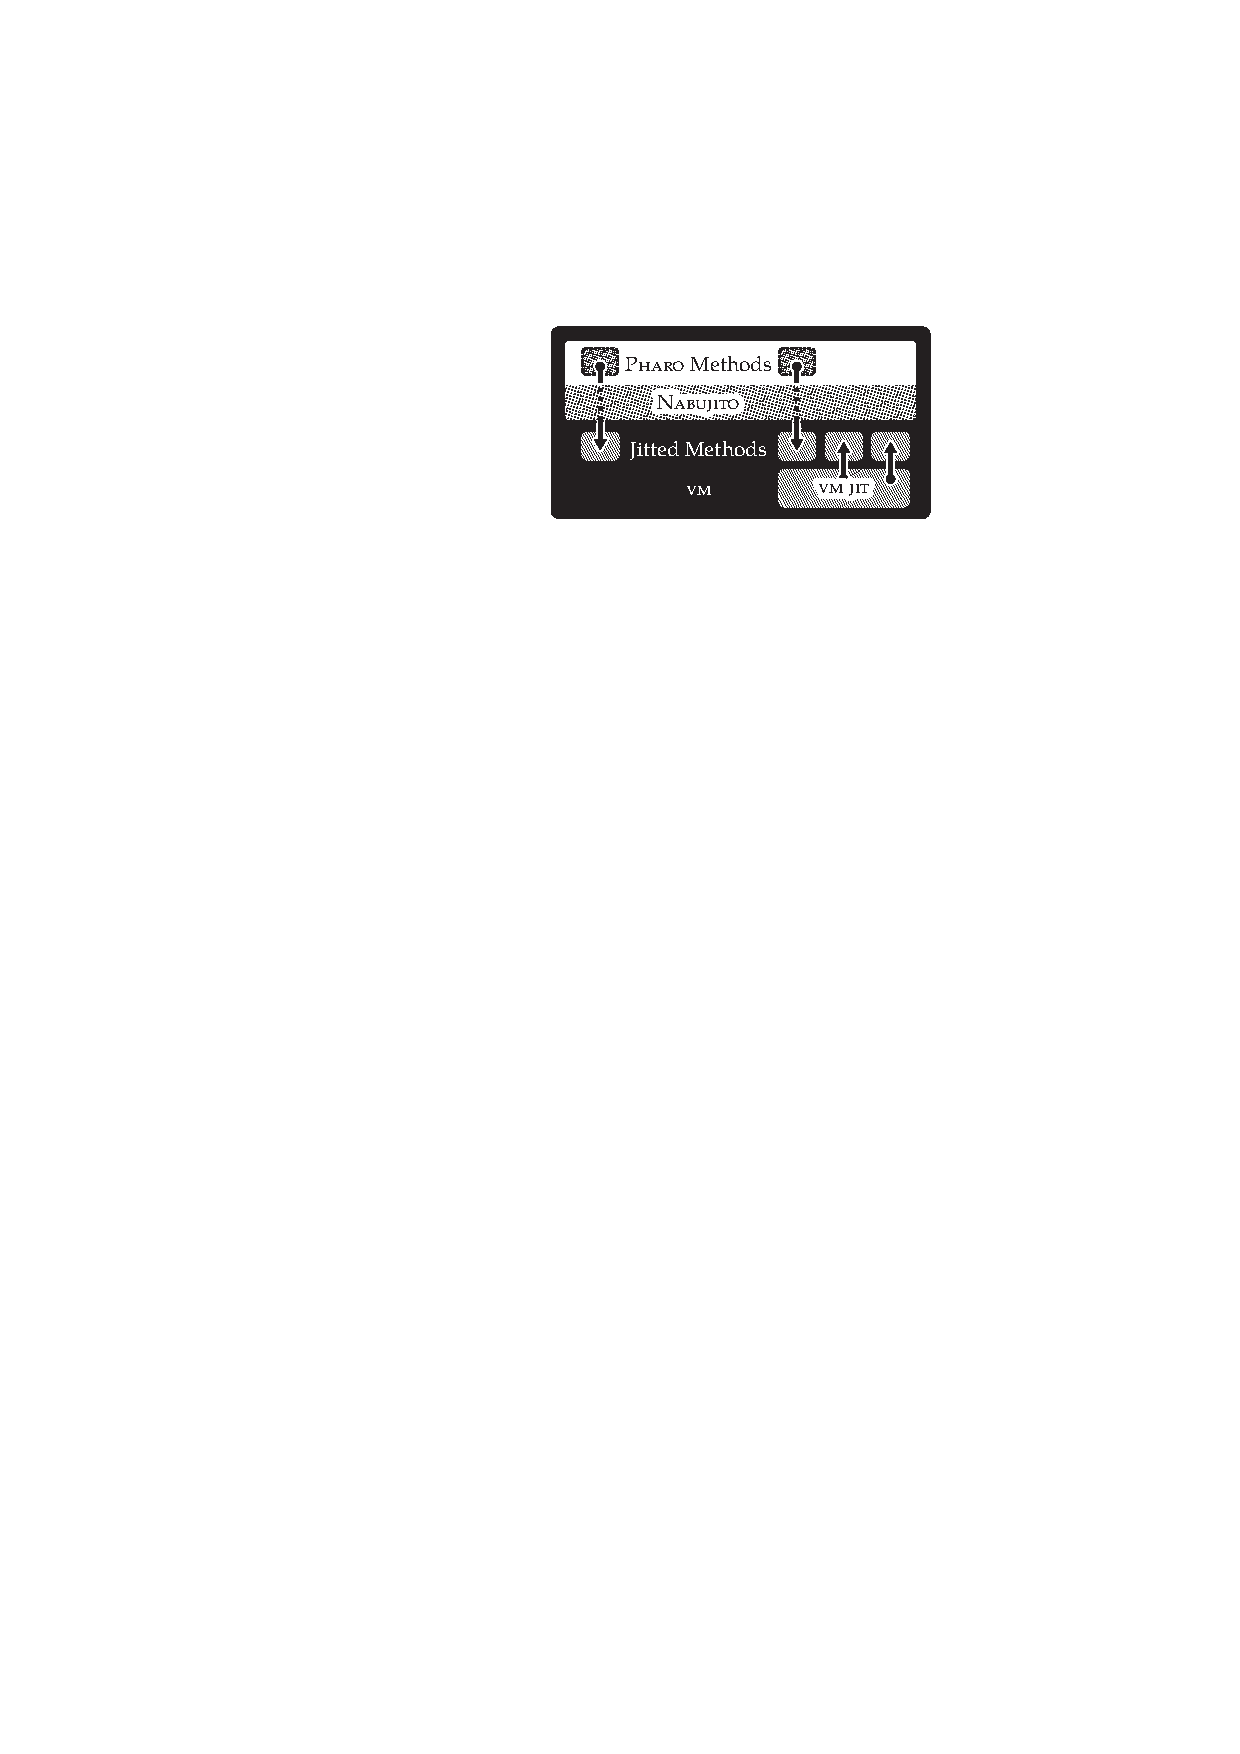
\includegraphics[scale=\imagescale]{nabujito-overview}
\end{figure}

\noindent In this section we present \NBJ, a \B-based approach for a language-side \JIT compiler.
\todo{Introduction}

% ---------------------------------------------------------------------------
\subsection{Background}
\seclabel{val-nabujito-background}
% ---------------------------------------------------------------------------

\NBJ goes even further than \WF using almost the same techniques.
However, instead of focusing on primitives, \NBJ generates native executable code for standard \ST methods.
Primitives tend to be more low-level, whereas \NBJ focuses on high-level \ST code. 


%----------------------------------------------------------------------------
\paragraph{The \JIT of the \PH \VM}
The \PH \VM (Cog) already comes with a \JIT that translates bytecodes to native instructions.
It transforms \ST methods into slightly optimized native code at runtime.
The main speed improvement comes from avoiding bytecode dispatching and by inlining certain known operations and primitives \cite{Ayco03a}.
The most complex logic of the \JIT infrastructure deals with the dynamic nature of the \ST environment.
Methods and classes can be changed at runtime and that has to be addressed by the \JIT infrastructure.
The \JIT compiler, by which we refer in this context to the transformation of bytecodes to native code, represents a small part of the whole infrastructure.
There exists more important stages as an additional register allocation pass to reduce the number of stack operations \cite{Mira99a,Mira11a}.
The existing \JIT infrastructure is implemented in \Slang \cite[Ch.\ 5]{Blac09a} as the rest of the \VM.

To understand the upcoming implementation issues of \NBJ we have to dive into the details of \PH's \JIT.
\PH uses a flavor of the \Cog \VM which evolved in several steps from a simple bytecode interpreter.
A successful and fast \JIT implies a \VM that uses the native stack.

The original \ST-80 blue book implementation foresees a spa\-ghet\-ti-stack where all contexts are normal objects on the heap.
This design simplifies the \VM implementation significantly since there is no special treatment necessary for blocks.
Also this makes it rather easy to implement \PH's feature to access the current context using the special \ttt{thisContext} variable.
However, the obvious down side of this implementation is the massive stress on the \GC.
For each message send a new context has to be allocated and on each return contexts have to be reclaimed.
It would naturally be more efficient to use the native stack which allows for cheap allocation and precise reclaiming of method context.
While this mapping can be done rather easily there are three properties of \PH that make this hard: blocks, non-local returns and the mentioned \ttt{thisContext}.
Eliot Miranda eventually succeeded to implement an efficient mapping scheme for the \Cog \VM that is based on the original work done by Peter Deutsch and Allan Schiffman \cite{Deut84a}.

Even so the basic concepts of the native stack mapping are easy to understand the final implementation is tricky details.
Real closures that outlive their outer method activation context make the mapping difficult.
At the same time all the reflective capabilities to modified the stack from within \PH have to be supported.
This, in return, limits the optimization opportunities.
\Cog chose a path in between where most reflective modifications of the stack are permitted.
However, in certain exotic edge cases the \VM does not support the operation.

After supporting the native stack the next optimization in line is the real \JIT infrastructure where the \VM generates native code on the fly.
In \Cog there is a bytecode compiler that generates a simple intermediate representation which then is used to generate the final native instructions.
The \IR makes it easier to support new platforms next to the default 32-bit x86 implementation.
\Cog applies minor optimizations like a simple register allocation strategy to lower the stress on stack usage.
The most underestimated optimization is the fact that all the native code for the jitted methods is stored in a compact separate memory region.
This lowers the chances of cache misses, an ever growing problem on modern \CPU architectures.

\figref{cog-memory} gives and overview of the memory separation used by \Cog.
%
\begin{figure}[h]
	\centering
	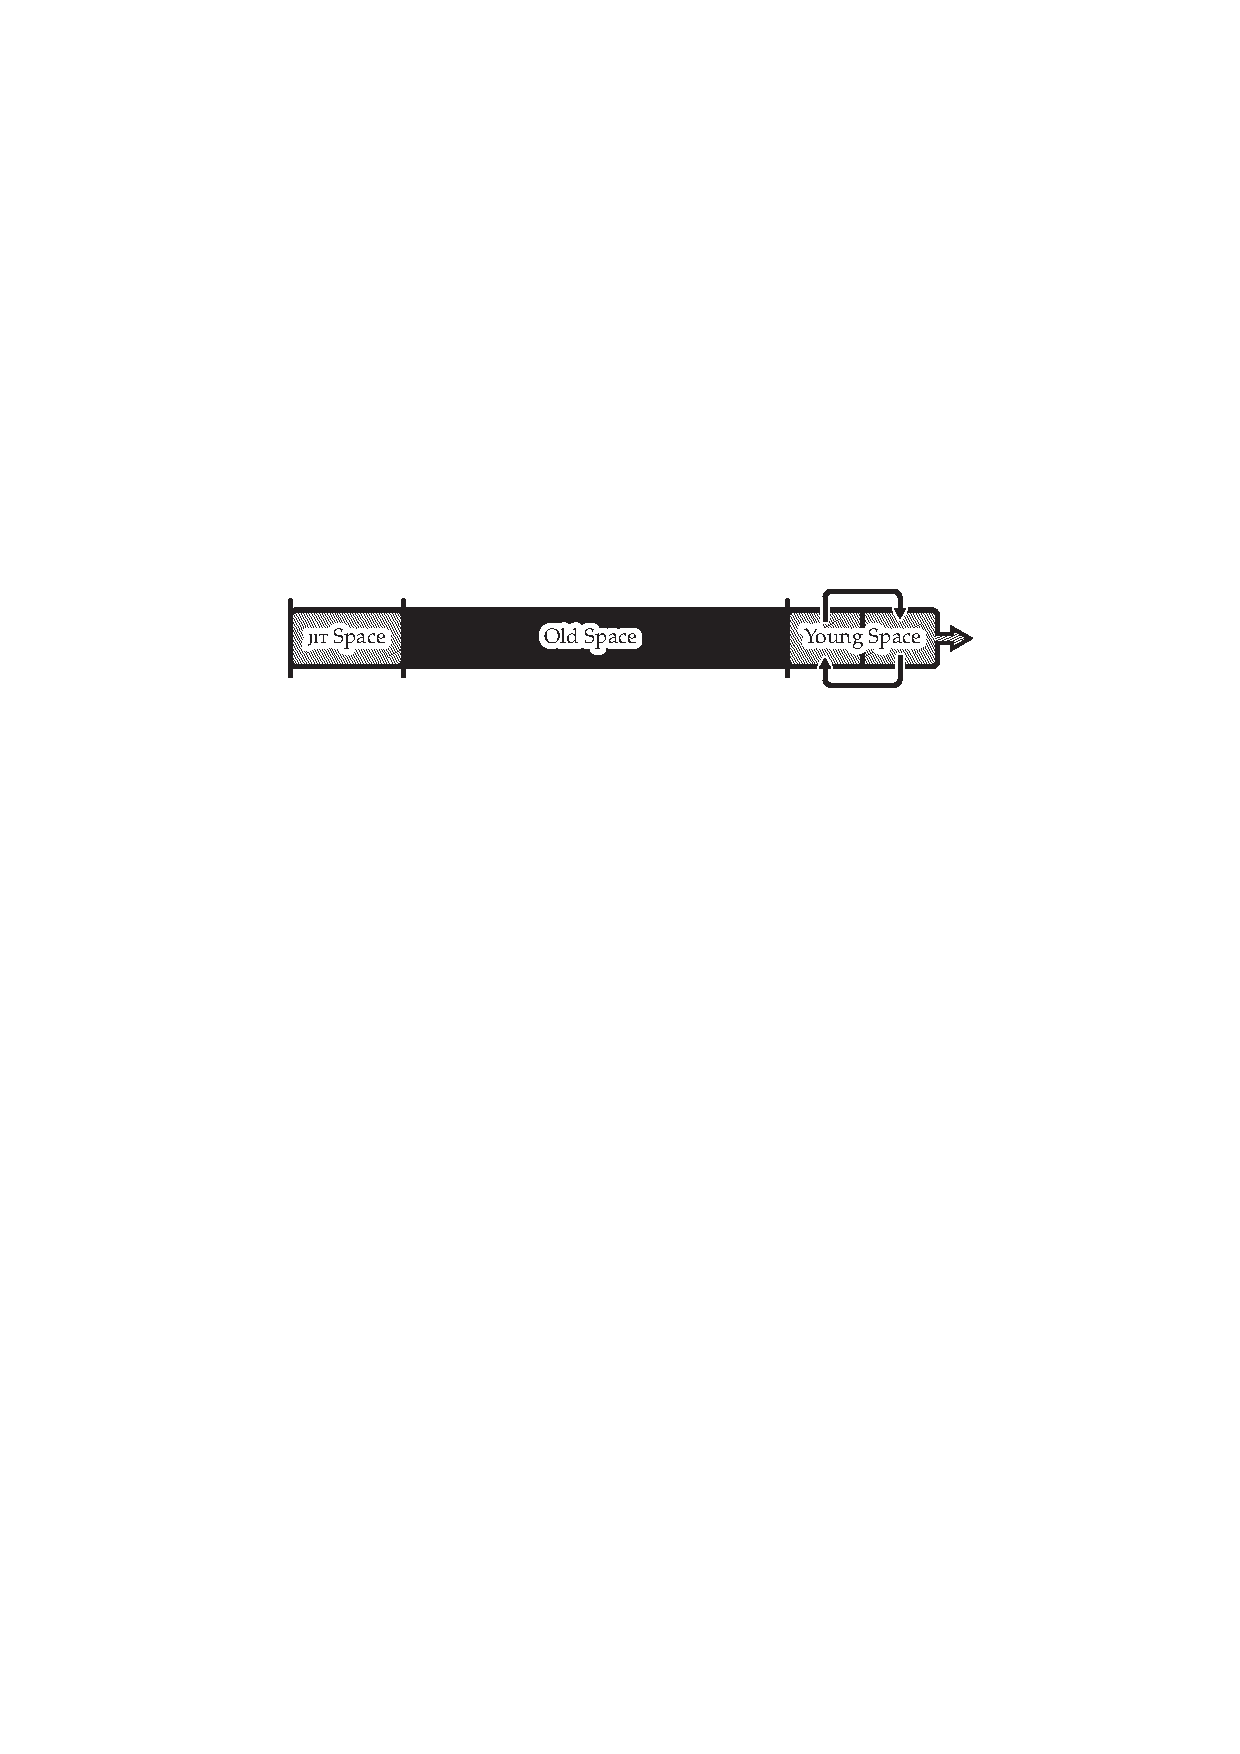
\includegraphics[scale=\imagescale]{cog-memory}
	\caption[\Cog Memory Model Overview]{\Cog Memory Model Overview: Fixed-sized \JIT space, slow changing old space and fast young space.}
	\figlabel{cog-memory}
\end{figure}
%
New objects are allocated in the young space which uses a fast semispace \GC with frequent reclaiming.
Objects that survive a \GC pass move to the old space where infrequent reclaims happen.
Separated from the two memory regions where normal \PH objects reside is the \JIT space dedicated for native code.
In \Cog the \JIT space has its own \GC strategy tailored to native code which is stored in a structure called \CogMethod.
Each jitted \PH method has a corresponding \CogMethod with native code which resides in the \JIT space.
The \CogMethod caches certain information such as the selector or number of arguments.
Again this improves code locality as all the frequently accessed information resides in the \JIT space.
\figref{cog-method} gives an overview of the \CogMethod.
We see that additionally to the cached meta information there is relocation information (method map) attached to the \CogMethod.
This is used to update object reference, typically to selectors, form the native code in sync with the objects that were moved in a \GC pass.
The same information is also used to update jumps to other native code in the \JIT space if the dedicated \JIT \GC performs a compaction.
%
\begin{figure}[h]
	\centering
	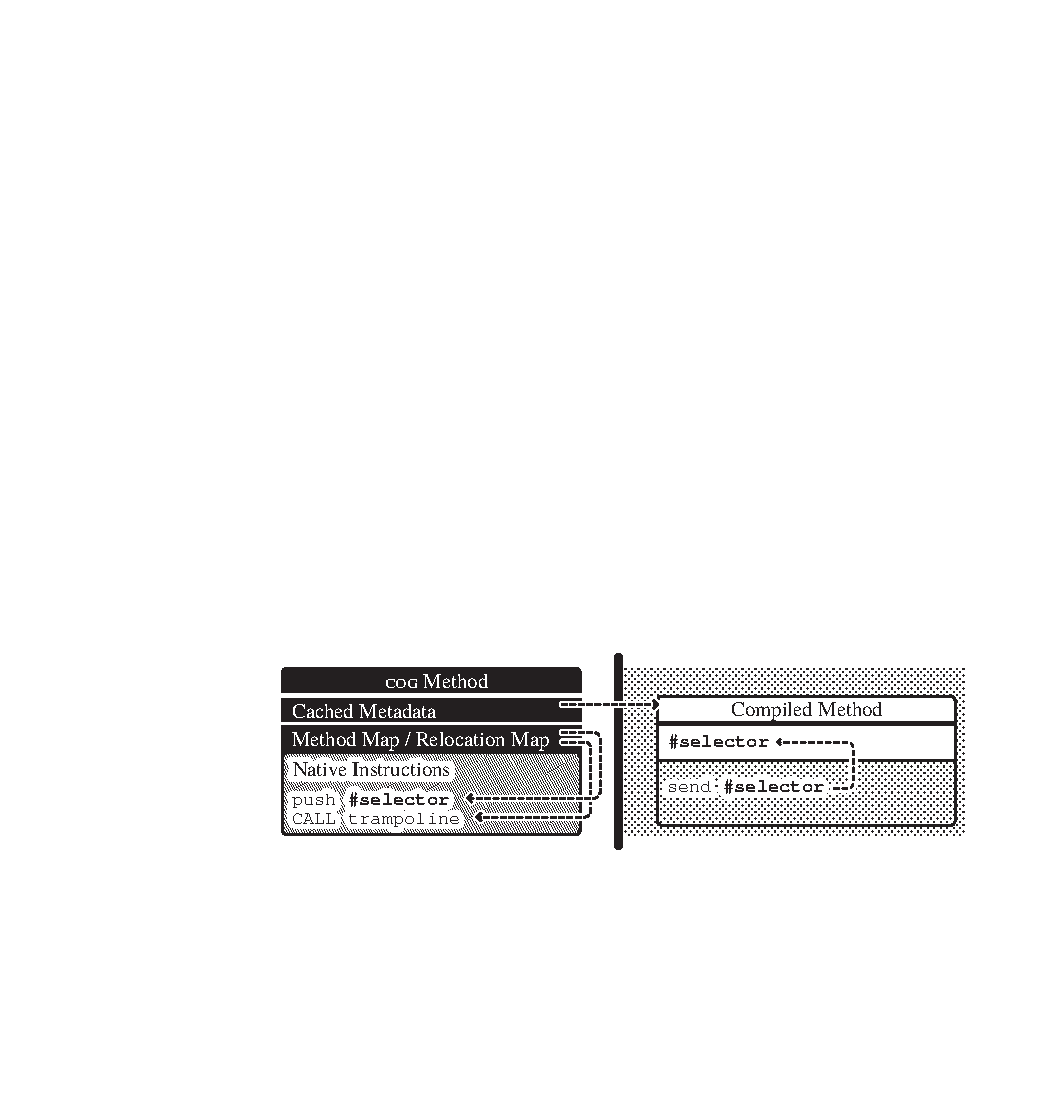
\includegraphics[scale=\imagescale]{cog-method}
	\caption[\Cog Method]{\Cog Method: Compiled method representation at \JIT-level residing in the \JIT memory space.}
	\figlabel{cog-method}
\end{figure}

\noindent So far we explained how \Cog uses native stack mapping for performance reasons and how the basic \JIT compiler works.
The limit the stress on the \CPU cache only the most used methods are jitted.
\Cog uses a hierarchy of inline caches to avoid the costly method lookup and checks if a method is already jitted or not.
Message sends from one jitted method to another hence happen with a very low overhead.
However, due to the limited size of the \JIT space that still means that infrequently used methods are evaluated using the existing bytecode interpreter.
\cb{the previous paragraph might be a bit dense, depending on the knowledge of the reader}
Since \Cog uses stack mapping this means that the C-based bytecode interpreter runs on the same native stack with two slightly different strategies.
For instance, typically the C stack depth is limited to a predefined constant, whereas the \PH stack can grow as big as the whole heap.
Which means that recursion in a \PH program is not a direct threat.
In the bytecode interpreter the language-side recursion is not directly present, since the interpreter only fetches and evaluates bytecodes in a loop.
Thus, switching from \JIT-mode to bytecode interpretation requires some additional work to avoid negative side-effects.
Essentially, \Cog separates the native stack for the \JIT and the bytecode interpreter.
Each time \Cog has to switch execution mode it goes through a trampoline routine.
The trampoline will exchange the two native stacks and jump to the proper location to continue the execution of the bytecode interpreter from the native \JIT mode or vice versa.
If \Cog would simply call back to the C interpreter a new stack frame would be allocated, notably on the existing native \JIT stack.
This stack frame would persist as the bytecode interpreter continues running normal \PH message sends.
\todo{reread}

%----------------------------------------------------------------------------
\paragraph{Limitations of \VM-level \JIT Compilers}
In the context of \NBJ we split the \JIT infrastructure into separate parts.
The major part is to have a \VM that uses stack-mapping.
In the case of a bytecode-based interpreter, we assume that the \VM provides routines to switch between a bytecode interpretation context and a low-level native execution context.
With \NBJ we move the \JIT compiler,the part that generates native code at runtime, from the \VM to the image.%, the part that generates native code at runtime, typically from bytecodes.
 Since the \JIT compiler is quite decoupled from the rest of the \JIT infrastructure we believe that a hard-coded static and low-level implementation is not optimal for several reasons:

\begin{itemize}
	\item Optimizing \ST code requires strong interactions with the dynamic environment.
	\item Accessing language-side properties from the \VM-side is hard.
	\item Changing the \JIT compiler requires changes at \VM-level.
	\item The \JIT reimplements primitives for optimization reasons resulting in code duplication.
\end{itemize}

\paragraph{Optimization Limitations for \PH}
In \ST methods tend to be very small and it is considered good practice to delegate behavior to other objects.
This implies that several common optimization techniques for static languages do not work well.
Dynamic method activation does not provide enough context for a static compiler to optimize methods.
Hence after inline caches and register allocation the next optimization technique is inlining.
However, inlining in a dynamic context is difficult and requires hooks at \VM-level to invalidate native code when the language-side changes.
Since in \PH, compiling a method to bytecode is handled completely with language-side code most of the infrastructure to get notified about method changes is already present.

\paragraph{Primitives in the Existing \JIT}
The existing \JIT reimplements the most used primitives at \VM-level.
This guarantees that the \VM stays as long as possible in the \JIT context (see \secref{benzo-jit-interaction} on page~\pageref{sec:benzo-jit-interaction}).
Additionally this enables new performance optimizations that for instance are hard to achieve with standard compliant C code.
A typical example is the integer addition which has to deal with overflow checks and conversion of tagged integers.
In \secref{val-waterfall} we describe how \WF suffers a similar constraint.
\WF manually defines such primitives in terms of native assembler instructions through the language-side \B interface.
\NBJ reuses the same optimized primitives so we rely on a single optimized definition which is shared among all native code libraries.

%----------------------------------------------------------------------------
\subsection{\NBJ Implementation}
\seclabel{val-nabujito-implementation}
%----------------------------------------------------------------------------
\NBJ is an experimental \JIT implementation which replaces the bytecode to native code translation of the existing \JIT infrastructure with a dynamic language-side implementation.
\NBJ is implemented mainly with a visitor strategy over the existing intermediate bytecode representation. 
Additionally we reimplemented vital native routines for the \JIT which are not directly exported by the \VM using \B. 
\cb{not sure if better to put down next to the \JIT limitation paragraphs...}
Nabujito relies on the following \VM-level infrastructure to manage and run native code for any \PH method:

\begin{itemize}[noitemsep,nolistsep]
	\item native stack management,
	\item routines for switching contexts,
	\item \JIT-level memory management for code segments.
\end{itemize}

\noindent The native stack mapping is an implicit requirement for an efficient \JIT.
Since this feature requires deep changes at \VM-level we can not alter or reimplement this at language-side.
However, the routines for switching between \JIT and non-\JIT execution context can be mostly reimplemented at language-side.
We only chose to implement a small subset of them with \B that were directly required for performing message sends.
Some of the helper routines' C-level addresses are easily accessible from language-side using \ttt{dlsym}.
Hence we reuse these for simplicity and only reimplemented the ones that are "hidden".
The last item we reuse, \JIT-level memory management, poses certain problems as we have little to no control over this from language-side.
There is no well-defined interface to interact with the \JIT from language-side in \PH.
However, to properly interact with the \JIT we have to tell it where references to language-side objects are located in the native code.
To overcome this limitation we chose to hack the current \VM to better interact with the \JIT.
More details on this topic follow in the following paragraphs.

\paragraph{\NBJ Dynamic Code Generation}
\NB mainly consists of a visitor over the bytecode-level \IR that is provided by the \PH compiler.
Additionally we reimplemented some of the aforementioned helper routines to switch execution context in the \VM.
The main difficulty of the \NBJ compiler is the missing interface to the \JIT.
For instance we did not have direct control on which methods in \PH are jitted or not, or to force-\JIT a method.
We added one additional primitive to be able to manually trigger \JIT compilation.

For standard methods \NBJ takes the bytecodes and transforms them with a visitor to native code.
It also applies simple optimizations such as creating low-level branches for \PH-level branching operations such as \ttt{ifTrue:}.
Optimizations for additional methods are all implemented flexibly at language-side.
Wherever possible, we reimplement the same behavior as the existing native \JIT compiler.

Eventually the native code is ready and \B attaches it to the existing compiled method.
At this point we benefit from the \JIT integration of \B itself.
As a reminder, we have shown in \secref{benzo-benzo} how \B-enabled methods are treated like normal primitive methods.
The \VM triggers a \B primitive which itself then jumps to the native code attached to the \B-enabled method.
By default the \Cog \JIT can only directly inline the native code for a known set of primitives.
As we have shown in \secref{benzo-jit-interaction} that the \Cog's \JIT was made aware of the special behavior of the \B primitive.
Hence, whenever a \B-enabled method is jitted its native code is directly accessible to the \JIT and inlined.
Thus we essentially remove the overhead of activating \B-enabled methods since we do not have to leave the \JIT execution mode.
As a result we call \B-enabled methods at the same speed as the existing \JIT.


\paragraph{Talking to the \JIT}
After the initial promising progress on building \NBJ on top of \B we soon realized that is does not suffice to just generate the equivalent native code as the \VM internal \JIT.
The first goal was to compile a simple method that just returns a constant integer.
Even at this stage it became apparent that there is a missing interface to the \JIT.
To explain that we have a look at the standard stack frame setup of a jitted method in \Cog shown in \lstref{val-nabujito-cog-frame}.
%
\begin{numstcode}[
	caption={\Cog \JIT Stackframe Setup},
	label={lst:val-nabujito-cog-frame}]{7}
push EBP
mov  EBP, ESP
push 0x1f452b00<CogMethod>
mov  EBX, 0x1f500004<nil>
push EBX
push EBX
\end{numstcode} 
%
After finishing executing these setup instructions the stack frame looks as depicted in \figref{val-nabujito-cog-stack-frame}.
%
\begin{figure}[h]
	\centering
	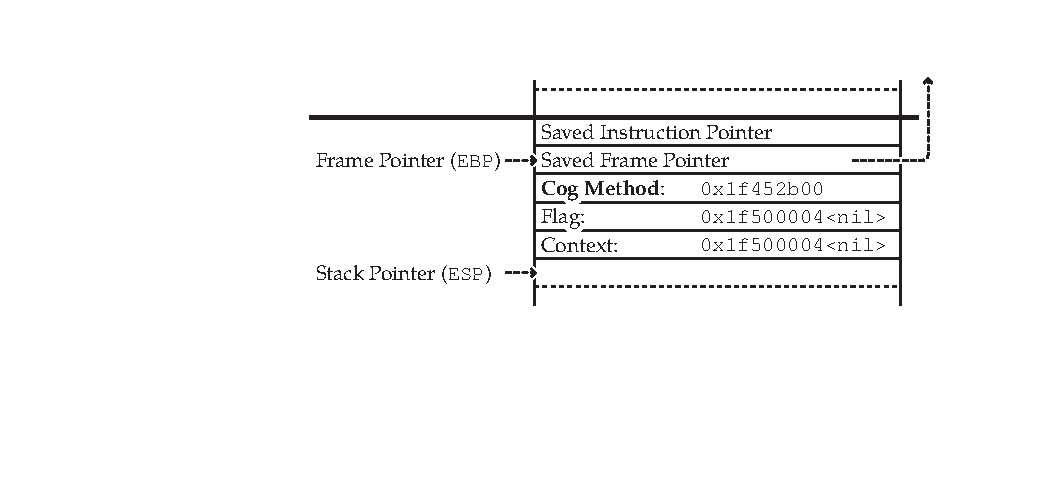
\includegraphics[scale=\imagescale]{cog-stack-frame}
	\caption{\Cog Stack Frame Header}
	\figlabel{val-nabujito-cog-stack-frame}
\end{figure}
%
As we can see there are already two references to \ttt{nil} in the stack frame header.
Already these two references pose a problem in a simple \NBJ setup, but for now we focus on the reference to the \CogMethod.
As we explained earlier the \CogMethod is a meta object at \JIT-level to make certain information of \PH methods faster accessible.
The \VM currently keeps a pointer to the class, the selector or the number of arguments cached in there.
Having the information there improves locality and make the assembler code required for the frequent querying simpler.
Going back to the native code in \lstref{val-nabujito-cog-frame} we see that we need the final address of the \CogMethod for the frame setup.
However, at the moment where \NBJ generates the native code the target method is not yet jitted.
This again implies that the corresponding \CogMethod has not yet been allocated by the \JIT.
And since the native code has to be installed in the \JIT we inevitably have to wait for \NBJ to finish compilation, we are stuck.

Instead of directly putting the absolute address of the meta-object in the native code we add a call to a helper routine which will patch the original code on the first activation.
We can do so since we know the following things:
\begin{itemize}[noitemsep,nolistsep]
	\item \CogMethod has a fixed size known upfront,
	\item we know the relative offset of the jitted method's instruction to the start of its \CogMethod,
	\item we can access the instruction pointer with a helper routine.
\end{itemize}
%
\noindent With this information we modify \NBJ to generate the modified frame setup show in \lstref{val-nabujito-frame-setup}.
%
\begin{numstcode}[
	caption={\NBJ Stack Frame Setup},
	label={lst:val-nabujito-frame-setup}]{7}
push EBP
mov  EBP, ESP
mov  EAX, 0x643d02e<pushCogMethodHelper>
call EAX
\end{numstcode}
%
In the \ttt{pushCogMethodHelper} we access the instruction pointer from where the call happened in the stack frame setup and deduce the start of the \CogMethod.
Once the address of the \CogMethod is retrieved the \ttt{pushCogMethodHelper} patches the \ttt{MOV} and \ttt{CALL} instruction in the jitted method.
The result is shown in \lstref{val-nabujito-patched-frame-setup}.
%
\begin{numstcode}[
	caption={\NBJ Patched Stack Frame Setup},
	label={lst:val-nabujito-patched-frame-setup}]{7}
push EBP
mov  EBP, ESP
push 0x1f452b00<CogMethod>
nop
\end{numstcode}
%
By using this indirection we circumvent the missing interface to the \JIT.
The helper routine only imposes a one-time overhead, however we slow down the final execution of the \NBJ method by a single \ttt{NOP} instruction.
Yet, looking at the \Cog stack frame in \figref{val-nabujito-cog-stack-frame} we only dealt with finding the reference to the \CogMethod.
So far we left out the \GC interaction at \JIT-level, which leads us to the following paragraph.

\paragraph{Overcoming the Missing \VM Interface for the \JIT}
\Cog embeds references to normal \PH objects in its jitted methods.
Most often this is the case for the symbols used as selectors in message sends.
This is different from the indirect approach used in compiled methods for the bytecode interpreter.
There all objects used in the method are stored in a separate literal array and referenced by an index.
Hence the bytecode can stay very compact and more importantly does not have to be updated on each \GC pass.
While for space consumption was the only concern on the early \ST implementation the \JIT only focuses on performance and thus avoids as many indirections possible; hence the use of direct references in the \JIT.
That implies that unlike the bytecodes, the \JIT code is no longer independent of the location of the referenced objects and thus has to be updated on each \GC pass.
Additional to moved objects no the \PH heap, the \JIT space itself moves a \CogMethod when compacting native code.
Hence the \GC has to also be aware of jumps and reference to another \CogMethod inside the native code.
In \Cog this additional information is stored in the \CogMethod itself, called method map.
It contains simple entries which describe the location of jumps, calls, references to other \CogMethod objects and references to \PH objects.
%
\begin{figure}[h]
	\centering
	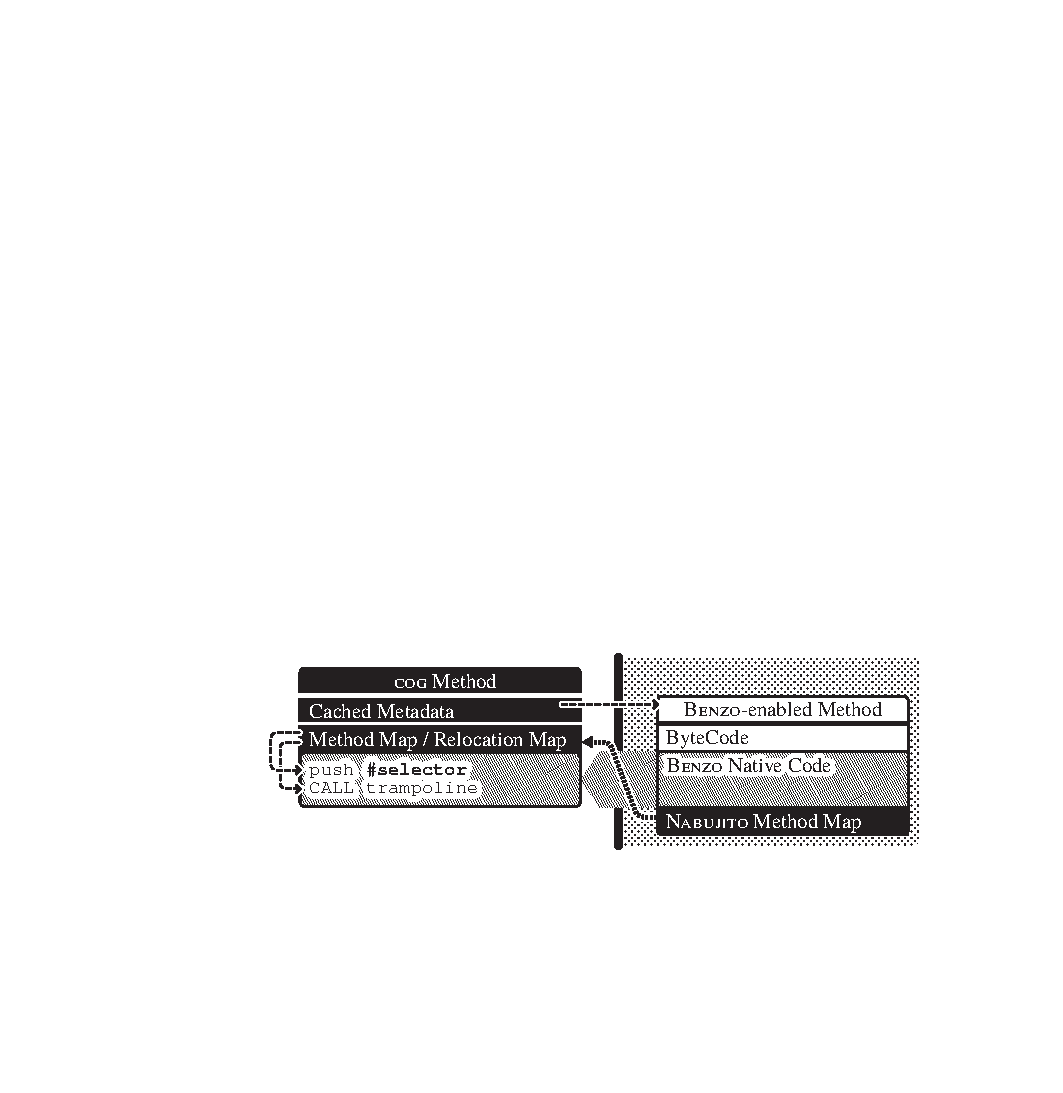
\includegraphics[scale=\imagescale]{cog-method-map}
	\caption{\Nabujito-generated Relocation Maps}
	\figlabel{val-nabujito-cog-method-map}
\end{figure}
\todo{integrated figure}

The low-level design of \Cog has significant implications on how \NBJ has to interact with the \VM.
\NBJ has to provide the location of every reference and jump inside the native code.
With the design of \NBJ so far, this is not directly possible.
So far \NBJ directly copies the native code from the \B-enabled method to the \CogMethod.
Hence, \NBJ ignores all the additional information required for the \JIT to work properly.
To comply with the \JIT we implemented a custom primitive for \NBJ with custom \JIT support, essentially creating a fork of the \VM.
The newly added primitive is a copy of the existing \B primitive with \JIT support.
However, the \NBJ adds support for the \CogMethod relocation maps.
At language-side the \NBJ compiler stores a relocation map as the first literal in the compiled method. \todo{make sure to implement it this way}
In the customized \JIT code for the \NBJ primitive we read this relocation information and forward it to the \Cog \JIT infrastructure.
Essentially we replicate the information of the \JIT-level \CogMethod inside a \B-enabled \PH method.

% -----------------------------------------------------------------------------
\subsection{\NBJ Validation}
\seclabel{val-nabujito-performance}
% -----------------------------------------------------------------------------
After explaining the implementation details and challenges of \NBJ we present a performance validation of our language-side \JIT compiler prototype.
Our current prototype implementation is not complete yet, we envision that the final compiler will produce the same native code as the existing \JIT of the \Cog \VM.
Based on that idea we focus our evaluation mainly on the language-side code generation.
Even though the underlying \B infrastructure caches the native code, the compilation step itself is several magnitudes slower than the native \JIT version.
Hence we first evaluate in detail the compilation speed of \NBJ, and only in the second part we focus no the real execution speed of the generated native method.
\todo{make sure we implement this claim}

% -----------------------------------------------------------------------------
\subsubsection*{Compilation Time}

In this first part of the performance evaluation for our \B-based \JIT compiler we focus on the language-side code-generation part.
\NBJ essentially generates the same native code as the \VM-level \JIT, hence there is no performance difference at evaluation time.
However, \NBJ is clearly slower during the warm-up phase.
Compilation of the native instructions will take considerably more time compared to the \VM-level implementation of the same bytecode to assembler transformation.
The cost of transforming the bytecodes to native code at \VM-level can be measured in native instructions, whereas the unit at language-side is bytecodes.
However, we point out again, that this is a one-time overhead.
From the in-production experience of \NB, the \B-based \FFI (see \secref{ffi-evaluation}), we know that these costs amortized, especially for long-term applications.
Instead of focusing on the final performance of the generated code, we present the compilation time compared to the normal \PH bytecode compiler, which also resides at language-side.

\begin{table}[!ht]
    \centering
    \begin{tabular}{rS}
                      & {Compilation Time [ms]} \\\midrule
        \PH Compiler  & 71(1) \\
        \NBJ          & 73(1)
    \end{tabular}
    \caption[\NBJ Compilation Speed]{Compilation efforts of the standard \ST compiler in \PH and \NBJ for the a simple method returning the constant \ttt{nil}.}
    \tablabel{val-nabujito-performance-small}
\end{table}

\noindent In \tabref{val-nabujito-performance-small} we compare the compilation speed of the standard \PH compiler and \NBJ.
We measure the accumulated time spent to compile the method 1000 times.
The average and deviation are taken over 100 runs. 
The \PH compiler takes source code as input and outputs \ST bytecodes.
\NBJ takes bytecodes as input and outputs native code.

We see that in the simple case displayed in \tabref{val-nabujito-performance-small} \NBJ's compilation speed lies within the same range as the standard \ST compiler.
We expect that in the future we apply more low-level optimizations and thus increase the compilation time of \NBJ.
However, we have shown in the performance evaluation for \NB, the \B-based \FFI, in \secref{ffi-evaluation} that even a rather high one-time overhead is quickly amortized.
Furthermore with \ST's image approach the generated native code is persistent over several sessions.
A subsequent restart of the same runtime will not cause the \JIT to nativize the same methods it did during the last launch.
Hence our approach is even valid for short-timed script-like applications as most of the methods will already be available in optimized native code from a previous run.

% -----------------------------------------------------------------------------
\subsubsection*{Per Method Comparison}
\todo{choose simple enough methods that we can compile with nabujito: currently only + works}


% -----------------------------------------------------------------------------
\subsection{Related Work}
\seclabel{val-nabujito-related-work}
% -----------------------------------------------------------------------------
There is a vast amount of scientific literature when it comes to \JIT optimizers.
However, they focus on the optimization opportunities itself such as different compilation strategies or an efficient \GC interaction.
In the context of our work the compiler-based optimization are of second importance since we focus on the hybrid nature of a system that interacts with the low-level \VM world.

Jan Vran\'{y} et al. present a \ST with an explicit meta-object-protocol allowing for method lookup customization at language-side\cite{Vran12a}.
Their customized \ST/X \VM has an extended lookup mechanism where each class can specialize the lookup with a user definable \ttt{LookupObject}.
Hence for each message send the \VM first checks if the receiver's class provides a \ttt{LookupObject}.
By default this is not the case and the \VM falls back to the standard hierarchical \ST method lookup which is hard-coded in the \VM.
However, if the receiver class returns a proper \ttt{LookupObject} the \VM delegates the lookup to this user-defined object.
The \ttt{LookupObject} is invoked with context information about the message send including access to the low-level lookup cache.
While the other context information is important for new lookup schemes, the exposed cache provides an simplistic interface for the \JIT.
If the language-side lookup uses the provided cache it is still possible to implement efficient caching at \VM-level.
\todo{I don't think there is anything closer?}


A similar, albeit simpler approach, was provided in the research \ST \VM \P \cite{Verw12a}.
There the message lookup is fully implemented at language-side, but unlike the \ST/X solution only the context information required for a standard \ST lookup is provided.
More explicitly, \P does not provide access to an internal cache which could be used for speeding up more elaborate lookup customizations.

The two projects presented only implicitly deal with the \JIT interaction.
However, they provide evidence about high-level customizations for a part of the execution.
In both projects it is possible to dynamically customize a static core \VM concept.
While it is possible to modify the lookup mechanism in many \VM generation frameworks, this does not extend to the runtime.



% -----------------------------------------------------------------------------
\subsection{\NBJ Problems and Future Work}
\seclabel{validation-nabujito-problems}
% -----------------------------------------------------------------------------
\paragraph{Hidden \VM Internals}
The major obstacle found while implementing \NBJ is the lack of a language-side interface to the \JIT.
In \secref{val-nabujito-implementation} we already showed how we circumvented most of the limitations.
Our final conclusion was to extend the \VM and add a customized primitive with its own \JIT support.
Strictly speaking this is against the principles of the \B framework, where tools should be implemented transparently at language-side.
Even though the \NBJ is mainly implemented in \PH, the required \VM modifications result in the problems already described in \secref{benzo-vm-extensions}.
\VM extensions tend to be less maintainable, eventually \NBJ will take the same path as many other research \VM projects based on \PH and stay unmaintained until the \VM becomes incompatible.

Most of the problems described for \NBJ are being addressed with \Sista, a new adaptive \JIT compiler for the \Cog infrastructure. 
Until now the \JIT compiler for \Cog is completely written in \Slang and thus frozen at \VM compilation-time.
\Sista takes a different approach by implementing most \JIT optimizations at language-side.
Though the underlying approach is very different from \NBJ.
\Sista will require a new \VM that supports querying the status of the inline caches from \PH code.
Based on the retrieved information \Sista will apply standard optimization techniques like inlining.
Instead of directly generating native code at language-side \Sista will encode additional information in an extended bytecode set.
The \VM is then capable of extracting the necessary information to generate optimized native code.
\Sista essentially avoids the problems we described in \secref{val-nabujito-implementation} which occur when directly injecting native code into the \JIT machinery.
\Sista's flexibility lies between the current \JIT present in \Cog and the \NBJ prototype.

\paragraph{Debugging Cycle}
While working on \NBJ we encountered the same debugging limitations found in the other \B applications.
However, the interaction with the existing \JIT required already substantial debugging efforts, mostly at assembler-level.
Hence, \B's missing high-level debugging facility does not have a big impact on the general development of \NBJ.
The main issue is that the \VM itself lacks separate tests for the \JIT infrastructure.
Even so the \Cog branch supports a high-level simulator for running the \JIT this is currently not supported under \PH.
Additionally the \VM lacks dedicated tests for the separate parts of the \JIT infrastructure.
However, with the previously mentioned \Sista project, efforts are being made to enable the existing \VM debugging infrastructure on \PH, along with dedicated tests.

\paragraph{Missing Optimizations}
One major performance optimization missing in both, the original \PH \VM-level \JIT and \NBJ, is inlining. 
By inlining we are able to create methods that are potentially big enough for optimizations.
However, inlining is a difficult task in a highly dynamic language such as \ST or \Self \cite{Cham89a}. 
Efficient inlining can only be performed with sufficient knowledge of the system. 
Accessing this high-level information from within the \VM is cumbersome and requires duplication of language-side reflective features.
The \JIT lives on the same level as the information it needs relying on the already present reflective features of \ST.


% ===========================================================================
\newpage
\section{\B Applications: Outlook and Summary}
% ===========================================================================


In this chapter we presented two \B-based research projects: dynamic primitives and a language-side \JIT compiler prototype.
We have shown in \secref{val-waterfall} how the \WF toolchain allows us to modify \PH primitives on the fly. 
\WF uses the existing \VM source code written in the \ST subset \Slang, thus simplifying the modification of existing primitives.
Using the same \Slang sources \WF is also capable of compiling whole plugins on the fly.
In \secref{val-waterfall-performance} we showed that \WF outperforms a pure \PH-based solution when instrumenting primitives.
\WF is up to one magnitude slower than native \VM primitives leaving room for optimizations.

In the second part we presented \NBJ a language-side \JIT compiler that uses \B for the code generation part.
Even though \NBJ looks promising, the current implementation does not go beyond the stage of a prototype.
We identified that a reasonable \B-based \JIT implementation requires a well-defined interface to the otherwise isolated \JIT.
We have shown that the compilation time from bytecode to native code takes the same time as the standard bytecode compiler.
However, from a real-world point of the view the current \NBJ setup is insufficient since it requires a customized \VM.
A sufficient stable \JIT interface is required to efficiently implement \NBJ.
\todo{SISTA}

Both of these applications are a further validation of the \B framework and the concept of an open language-runtime without a clear distinction between language-side and \VM-side.
With the current setup we are capable of hosting important \VM parts such as non-essential plugins and primitives to the language-side.
However, again we encountered the typical limitations of the \B framework: missing high-level debugging and hard-coded assembler assumptions.
As before we refer to the suggested \B improvement presented in \secref{benzo-problems}.

While working on \NBJ we realized that most important primitives two different implementations.
Once there is the default implementation written in \Slang using the C stack.
Then there is an additional assembler-level implementation for the \JIT.
This is necessary to avoid frequent context switches for primitives.
However, with the current \B infrastructure it might be possible to use the same definition of the primitive for both usages and thus reduce code duplication.

The two \B research applications in this chapter have shown the limitations of our framework.
This will conclude our validation of \B itself and we will focus on the future work to extend \B's capabilities in the following chapter.

% =============================================================================
\ifx\wholebook\relax\else
    \end{document}
\fi